\documentclass{article}
\usepackage{graphicx} % Required for inserting images
\usepackage{hyperref}
\usepackage[section]{placeins}
\title{\underline {\textbf{Summer 2023 Research Summary}}}
\author{Jaehah Shin}
\date{May 15th 2023 ~ TBA}
\begin{document}
\maketitle
\section{About the Author}
\quad
My name is Jaehah Shin.
This project is the summer research project that I am currently working on.
I will be second year student this fall in the University of Toronto and I am studying Engineerign Science.
In third year, Engineering Science student will get to choose their major, and I am planning to choose the Robotics major.
I am interested in the field of robotics, and I am planning to study more about the robotics in the future.
I am currently working in the Prof.Franklin's lab in the University of Toronto. 
More information can be found in the following link. \href{https://franklinresearch.ca}{Prof.Franklin's Lab} 
I am currently working on the project that is related to the Induced Local Thermal Hyperemia Coupled with Laser Doppler Flowmetry to Assess Endothelial Function.
The following section will describe the overview of the project that will be worked on this summer. 
\section{Proposal of the Project}
PDF file on the next page is the overview of proposal of the project that I am currently working on.
\begin{figure}[htpb]
    \centering
    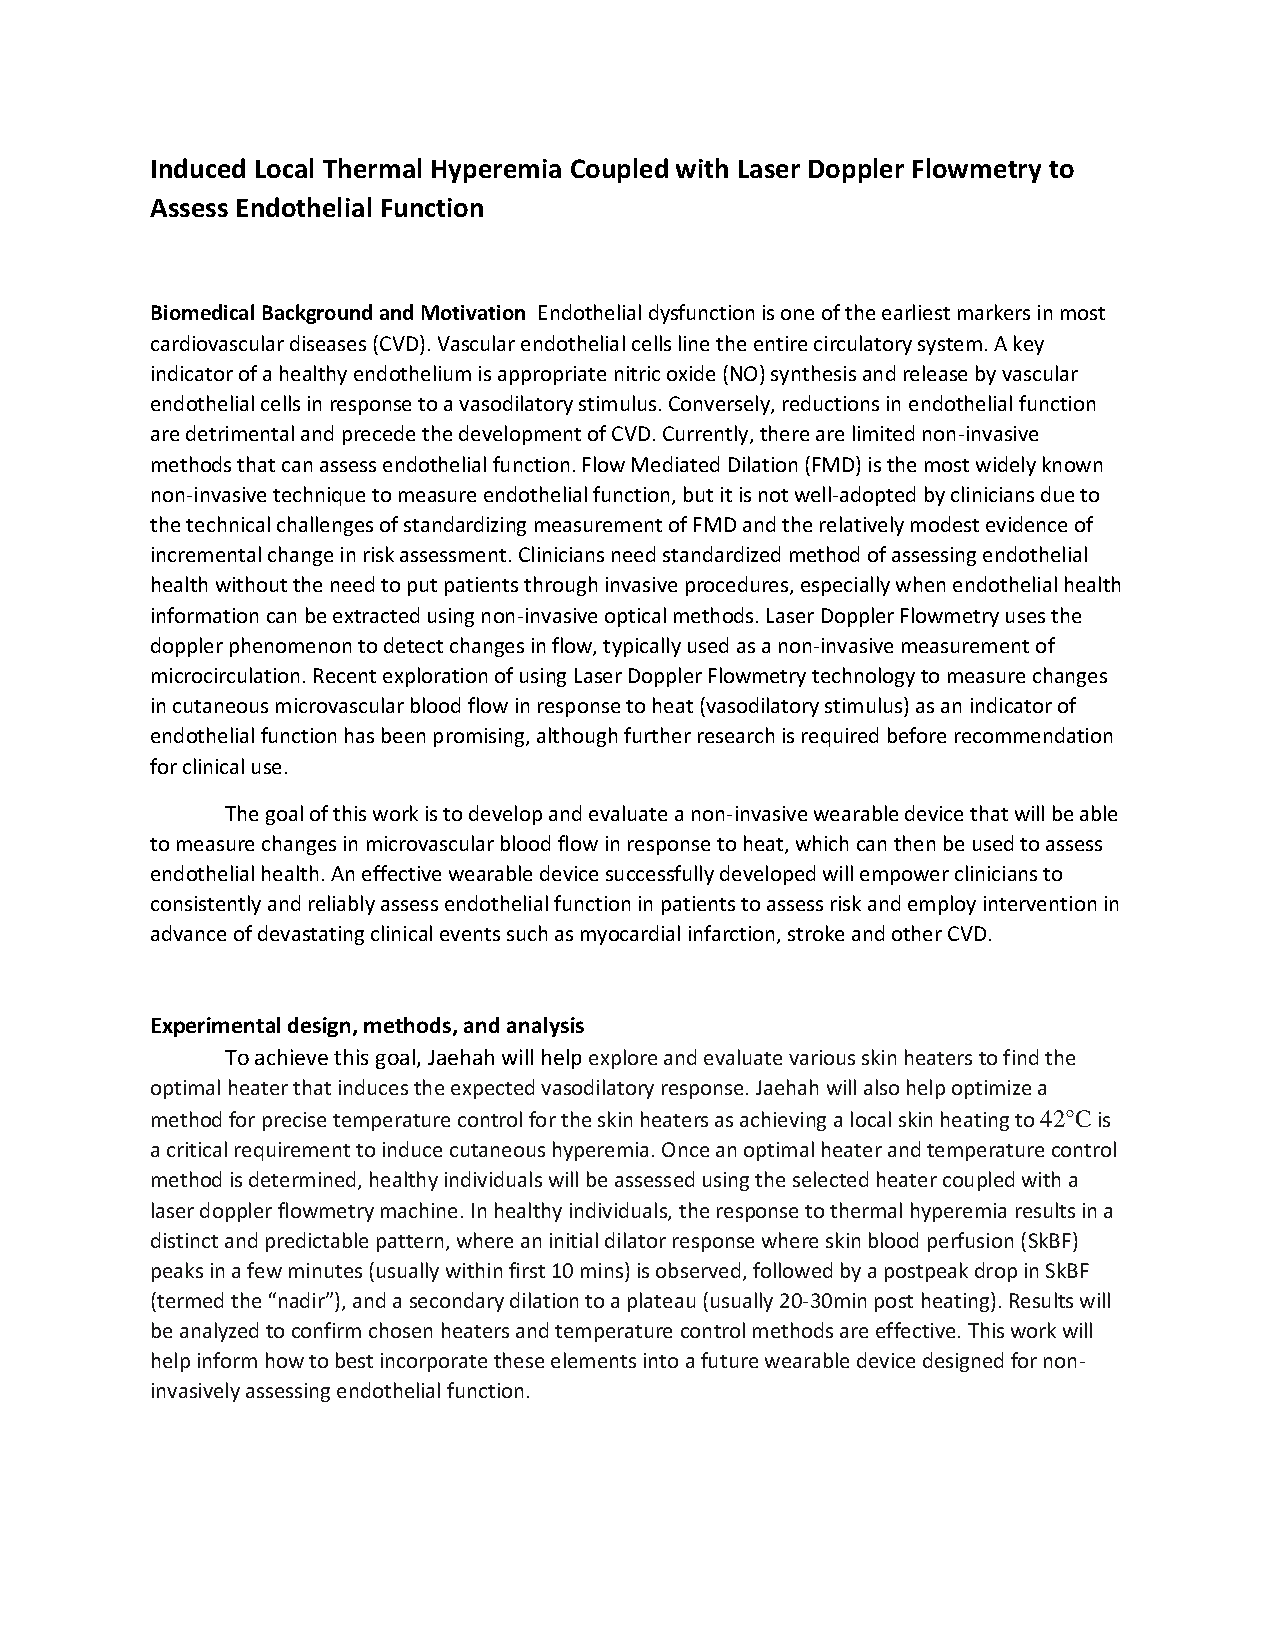
\includegraphics[width=1.1\textwidth]{Jaehah summer research proposal.pdf}
    \caption{The overview of the \texttt{Summer Research Proposal}}
    \label{fig:s_r}
\end{figure}

\section{About the thermister}
    On May 15th, my job was to learn bout the thermister, and find out how to use this.
Therefore, I did some research about the thermister.

We have all the values for 40.0 degress and 45.0 degrees in the table. 
Therefore we can use this table to cacluate those two temperatures. 
Aim is just to calculate the temperatures in general for lab purposes.

As the resistance of thermister is 10kohm, therefore, resitance of 
wire is negligible.
Thermister doesn't actually read the temperature. 
This reads the resistance of the thermister changes with temperature.

The thermister used in this project is TDK B57230V2103F260 which has 10k ohm
This is NTC thermister therefore, it has negative temperature coefficient thermistors.
Resistance decreases as temperature rises. 
this is due to the increase in the number of conduction electrons energized by the thermal
agitation from the valance bond. 
Actually, using the termistor is not the best for the accuracy of the temperature.
Since we measure the change of the resistance first and then convert it to the temperature.
Therefore, there are possible errors in the measurement.

However, there is the equation that can calcualte the temperature throuogh the resistance.
Then also the Arduino code can solve that equation. 
That equatino is called as steinhart - Hart equation.

\section{Steinhart - Hart Equation}

\LARGE
\begin{equation}
    \frac{1}{T} = A + B\ln(R) + C(\ln(R))^3
\end{equation}
\\
\normalsize
where A, B, C are the constants that are determined by the thermistor and written on the datasheet.
\begin{itemize}
    \item T is the temperature in kelvin
    \item R is the resistance in ohms
    \item A, B, C are the constants that are determined by the thermistor
\end{itemize}

However, there was one big problem with this equation to solve the problem.
On the datasheet provided, there was no A, B, C values.
Therefore, there was only one way to solve this equations which is measuring the resistance at 
three fixed different temeperature. 
As there are three unknowns, we need three equations to solve for A, B, C.
For example, at 40.0 degrees, 45.0 degrees, and 50.0 degrees, we can measure the resistance.

And then compute the values to calculate for A, B, C, then
implement that equation with all the coefficients in the arduino code. 
However, as the lab bought the heater temperature controller, this method is not necessary anymore.
As the heater temperature controller has the thermister, it can read the temperature directly which is 
more accurate than the method that we were planning to use. 

\section{Heater Temperature Controller}
Lab bought the TC300 - Heater Temperature Controller from Thorlabs on May 18th.
\href{https://www.thorlabs.com/drawings/1a9e0ae31580f35c-5554A647-C109-6112-A4FC47A27614B988/TC300-Manual.pdf}{Document on Heater Temperature Controller}
Following part will be the sumamrized note for heater temperature controller on how to use it. 


\section{What is the possible effect of the heat on PCB panel?}
First of all, we need to know what is the PCB panel.
PCB panel is short for Printed Circuit Board.
As in this lab, the focus is how we can implement the heater into the PCB panel while measuring the temperature
of the skin with the heater, therefore, we need to know what is the possible effect of the heat on PCB panel 
as PCB panel and heater will be implemented together into the werarble device at the final stage of the project.

\subsection{What is the PCB panel?}
PCB panel is the board that is used to mechanically support and electrically connect electronic components.
This PCB panel is used almost in every electronic devices, and this will be used in the wearable device that we are 
going to implement at the final stagae. 






\section{...}

\section{..}


\href{}{Click This!} 

\end{document}
